\documentclass[tikz, border=1mm]{standalone}
\usepackage{tikz} 
\usetikzlibrary{arrows.meta}
\usepackage{pgfplots}

\pgfplotsset{compat=1.18}

\begin{document}

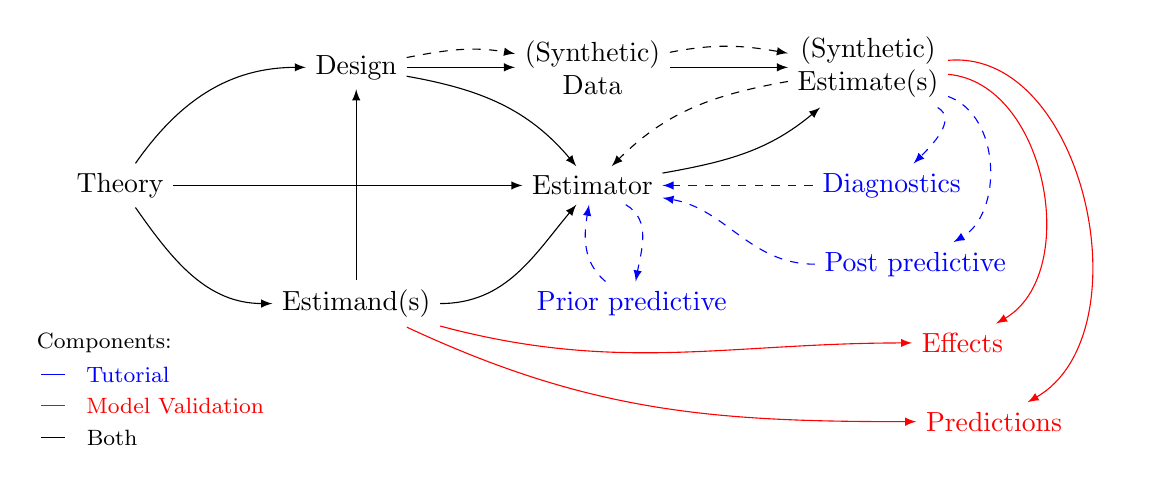
\begin{tikzpicture}

    % Legend
    \node[font=\footnotesize] at (-6.2,-2) (a) {Components:};
    \draw[font=\footnotesize, blue] (-7,-2.4) -- (-6.7,-2.4) node {};
    \node[font=\footnotesize, blue] at (-5.9,-2.4) (a) {Tutorial};
    \draw[font=\footnotesize, red] (-7,-2.8) -- (-6.7,-2.8) node {};
    \node[font=\footnotesize, red] at (-5.3,-2.8) (a) {Model Validation};
    \draw[font=\footnotesize] (-7,-3.2) -- (-6.7,-3.2) node {};
    \node[font=\footnotesize] at (-6.1,-3.2) (a) {Both};
    
    % nodes
    \node at (-6,0) (a) {Theory};
    \node at (-3,1.5) (b) {Design};
    \node at (-3,-1.5) (c) {Estimand(s)};
    \node[align=center] at (0,1.5) (d) {(Synthetic) \\ Data};
    \node at (0,0) (e) {Estimator};
    \node[align=center] at (3.5,1.5) (f) {(Synthetic) \\ Estimate(s)};
    \node[blue] at (3.8,0) (g) {Diagnostics};
    \node[blue] at (4.1,-1) (h) {Post predictive};
    \node[blue] at (0.5,-1.5) (i) {Prior predictive};
    \node[red] at (4.7,-2) (k) {Effects};
    \node[red] at (5.1,-3) (j) {Predictions};
    

    % paths
    \draw[-latex] (a) edge [out=55, in=180] node {} (b); % Theory -> Design
    \draw[-latex] (a) edge [out=305, in=180] node {} (c); % Theory -> Estimand
    \draw[-latex] (a) -- (e); % Theory -> Estimator
    
    \draw[-latex, dashed] (b) edge [out=11, in=170] node {} (d); % Design -> Synthetic data
    \draw[-latex] (b) -- (d); % Design -> data
    \draw[-latex] (b) edge [out=350, in=130] node {} (e); % Design -> Estimator
    
    \draw[-latex] (c) -- (b); % Estimand -> Design
    \draw[-latex] (c) edge [out=0, in=230] node {} (e); % Estimand -> Estimator
    \draw[-latex, red] (c) edge [out=345, in=180] node {} (k); % Estimand -> Effects
    \draw[-latex, red] (c) edge [out=335, in=180] node {} (j); % Estimand -> Predictions
    
    \draw[-latex] (d) -- (f); % Sample -> Estimates
    \draw[-latex, dashed] (d) edge [out=11, in=170] node{} (f); % Synthetic data -> Synthetic Estimates
    
    \draw[-latex] (e) edge [out=10, in=220] node {} (f); % Estimator -> (Synthetic) Estimates
    \draw[-latex, dashed, blue] (e) edge [out=330, in=80] node {} (i); % Estimator -> Prior
    
    \draw[-latex, dashed] (f) edge [out=190, in=45] node {} (e); % Synthetic Estimates -> Estimator
    \draw[-latex, dashed, blue] (f) edge [out=330, in=45] node {} (g); % (Synthetic) Estimates -> Diagnostics
    \draw[-latex, dashed, blue] (f) edge [out=340, in=30] node {} (h); % (Synthetic) Estimates -> Post
    \draw[-latex, red] (f) edge [out=5, in=30] node {} (j); % (Synthetic) Estimates -> Effects
    \draw[-latex, red] (f) edge [out=355, in=30] node {} (k); % (Synthetic) Estimates -> Predictions
    
    \draw[-latex, dashed, blue] (g) edge [out=180, in=0] node {} (e); % Diagnostics -> Estimator
    \draw[-latex, dashed, blue] (h) edge [out=180, in=350] node {} (e); % Post -> Estimator
    \draw[-latex, dashed, blue] (i) edge [out=140, in=260] node {} (e); % Prior -> Estimator
    
\end{tikzpicture}

\end{document}
